% ================================================================
% chapters/chapter6.tex --- RECONSTRUCTION
% ----------------------------------------------------------------
% Assemblé à partir des fragments retrouvés dans le project knowledge
% au fil de cette conversation, PAS une copie directe et vérifiée
% d'un seul fichier source. Fais un diff rapide contre ton fichier
% réel avant d'écraser l'original, par sécurité.
%
% CE QUI EST FUSIONNÉ ICI (déjà appliqué) :
%   - Objectifs : 2 phases au lieu de 3 (bloc itemize complet, pas
%     de "Lonely \item")
%   - Structure de la simulation : 2 phases (Exploration, Quiz)
%   - Mapping : SessionPayload -> SessionSubmitPayload, partout
%     y compris dans le use case "Soumettre une session"
%   - Cas d'utilisation "Vivre la simulation intigo" : renuméroté
%     sur 2 phases
%   - Code listing SimulationManager.cs : remplacé par le vrai
%     QuizManager.EndQuizAsync() (async/await, SessionSubmitPayload,
%     device token explicite) --- l'ancien listing montrait encore
%     un style coroutine + callbacks qui ne correspond ni à l'ancien
%     ni au nouveau code réel
%   - Conclusion du chapitre : nuancée ("en cours de finalisation"
%     au lieu de "fonctionne de bout en bout")
%
% CE QUI N'EST PAS TOUCHÉ (attend ta confirmation / tes vraies
% mesures) :
%   - Backlog du sprint 4 (tableau 6.2.2) : checkmarks inchangés
%   - Difficultés et solutions : inchangé
%   - Évaluation du sprint 4 : toujours "---", à remplir avec les
%     vraies mesures une fois testé sur casque
% ================================================================

\chapter{Itération~4 --- Simulation VR d'intégration Indigo Company}

\section{Introduction}

Cette quatrième itération représente le cœur fonctionnel de \tynassit{}~: la simulation VR
d'intégration des nouveaux employés d'\textbf{Indigo Company}. Cette scène plonge le nouvel employé dans un environnement 3D fidèle aux locaux d'Indigo, lui fait découvrir les différents départements accompagnés de narrations audio, puis évalue sa compréhension par un quiz. À la fin de la simulation,
les résultats sont automatiquement soumis à la plateforme \tynassit{}.

\section{Planification de l'itération~4}

Cette section définit les objectifs de la dernière itération, les tâches associées et
leur charge estimée.

\subsection{Objectifs}

\begin{itemize}
  \item Modéliser et optimiser l'environnement 3D Indigo Company dans Blender.
  \item Importer et intégrer l'environnement dans Unity~6.
  \item Développer les 2 phases de la simulation (exploration des locaux, quiz).
  \item Implémenter le système de quiz avec calcul automatique du score.
  \item Connecter la fin de simulation à \texttt{TynassApiClient.SubmitSession()}.
  \item Afficher les résultats dans le panel QuizResult.
\end{itemize}

\subsection{Tâches et estimations de l'itération~4}

\begin{table}[H]
  \centering
  \begin{tabularx}{\textwidth}{lp{2.8cm}Xcc}
    \toprule
    \textbf{ID} & \textbf{Titre} & \textbf{Description} & \textbf{MoSCoW} & \textbf{Charge estimée (j/h)} \\
    \midrule
    US-19 & Exploration des locaux &
      Environnement 3D Indigo (Blender + optimisation Quest~3) & \must{} & 8 \\
    US-20 & Quiz de fin de simulation &
      Simulation~: exploration + quiz & \must{} & 5 \\
    US-21 & Soumission automatique des résultats &
      SubmitSession → backend → visible dashboard & \must{} & 2 \\
    US-22 & Affichage des résultats &
      Panel QuizResult (score + critères) & \must{} & 1,5 \\
     US-23 & Navigation dans la liste des formations &
      Scroll VR joystick dans ModulesPanel & \could{} & 1 \\
    US-24 & Gestion des quiz &
      Interface entreprise~: création de quiz par formation & \must{} & 3 \\
    US-25 & Objectifs de formation &
      Milestones par employé (statut auto après session) & \should{} & 2 \\
    \midrule
    \multicolumn{4}{r}{\textbf{Total estimé}} & \textbf{22,5} \\
    \bottomrule
  \end{tabularx}
  \caption{Tâches et estimations --- Itération~4}
  \label{tab:backlog_s4}
\end{table}

\noindent US-19 à US-22, US-24 et US-25 ont été livrées~; US-23 reste en cours.

\section{Conception de l'itération~4}

Cette section présente la conception de la simulation~: la modélisation 3D de
l'environnement Indigo, la structure des deux phases, le système de quiz et la
correspondance des données transmises au backend.

\subsection{Modélisation 3D --- Blender}

L'environnement 3D d'Indigo Company a été modélisé dans \textbf{Blender} sur la base
des plans réels des locaux fournis par Indigo Company, puis exporté en FBX et importé
dans Unity~6.

Les optimisations appliquées pour Meta Quest~3~:

\begin{itemize}
  \item \textbf{Polygon count}~: inférieur à 500\,000 triangles pour la scène complète.
  \item \textbf{Textures}~: format ASTC 6x6 pour les grandes surfaces, ASTC 4x4 pour
    les textures détaillées.
  \item \textbf{Éclairage}~: \textit{baked lighting} (pas d'éclairage dynamique en
    temps réel), lightmaps calculées dans Unity.
  \item \textbf{Static Batching}~: activé sur tous les objets statiques pour réduire
    les draw calls.
  \item \textbf{Occlusion Culling}~: activé pour ne rendre que les objets visibles
    depuis la position courante.
\end{itemize}

\placeholder{Environnement Blender --- vue isométrique (à insérer)}

\placeholder{Environnement importé dans Unity~6 (à insérer)}

\subsection{Structure de la simulation}

 La simulation d'intégration Indigo (\texttt{indigo\_onboarding}) est organisée en \textbf{2 phases séquentielles}~:

\begin{enumerate}
  \item \textbf{Phase 1 --- Exploration des locaux}~: l'employé navigue librement dans les locaux d'Indigo Company et découvre huit zones interactives~--- les sept départements ainsi qu'une zone dédiée au responsable de département ---, chacune
présentée par un panneau d'information et une narration audio.
 \item \textbf{Phase 2 --- Quiz}~: questions à choix multiples évaluant la
    compréhension des informations présentées lors de l'exploration. Le nombre
    et le contenu des questions sont définis par l'entreprise depuis son tableau de bord.
\end{enumerate}

\begin{figure}[H]
  \centering
  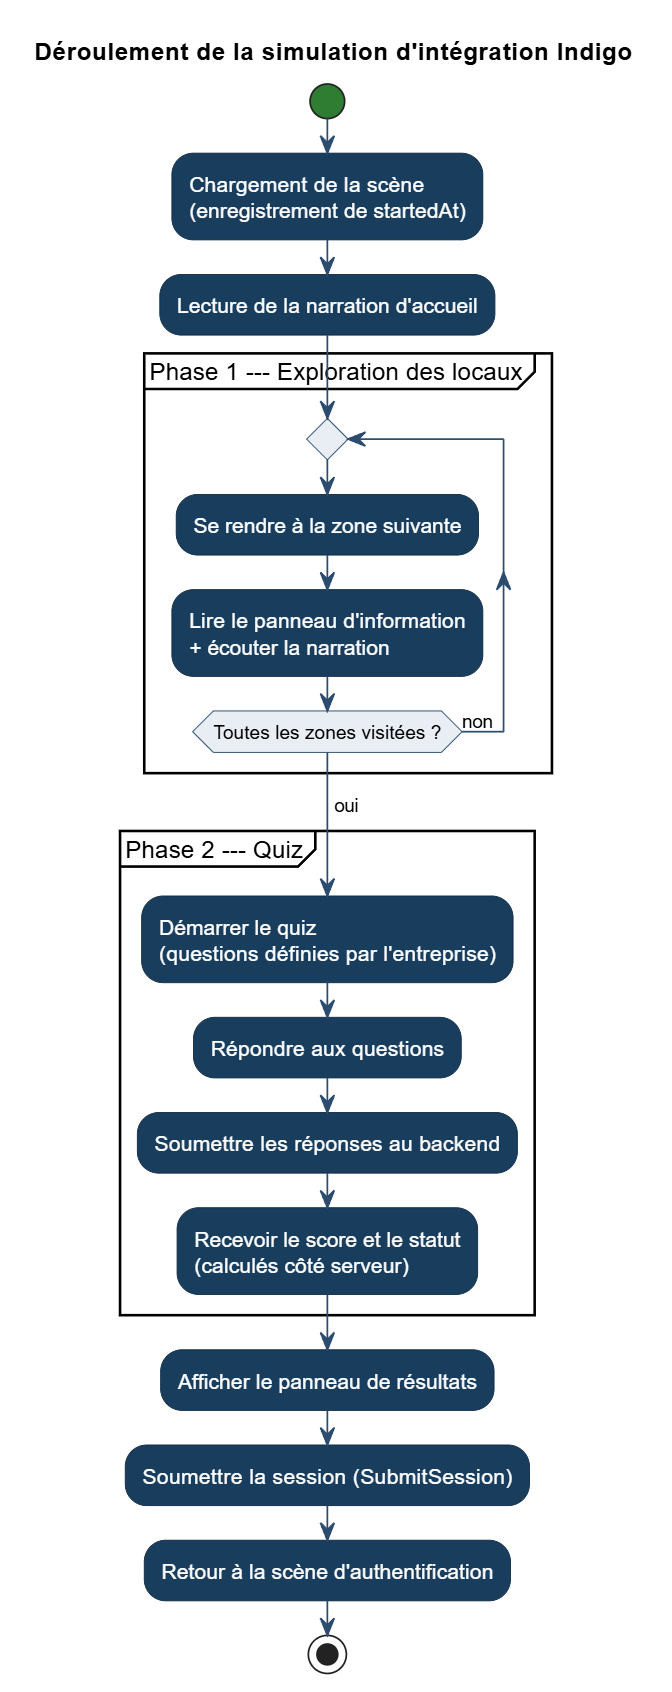
\includegraphics[width=0.7\textwidth]{../images/activiteSimulation.png}
  \caption{Diagramme d'activité --- déroulement de la simulation en deux phases}
  \label{fig:activite_simulation}
\end{figure}

\subsection{Système de quiz}

Les questions du quiz et leur nombre sont définis par l'entreprise cliente depuis son tableau de bord~; ils ne sont pas figés dans l'application. Le casque transmet les réponses de l'employé au backend via \texttt{POST /company/quiz/submit}~; le backend
les valide 
--- les bonnes réponses ne sont jamais envoyées au casque, ce qui empêche toute triche 
--- puis renvoie le score et le statut de réussite. Le score est calculé selon~:

\[
  \text{Score} = \frac{\text{QuizCorrect}}{\text{QuizTotal}} \times 100
\]

\[
  \text{passed} = \text{Score} \geq \text{passingScore}
\]
où \texttt{passingScore} est le seuil de réussite défini par l'entreprise, fixé à 70~\% par défaut.
\subsection{Mapping AppSession → SessionSubmitPayload}

\begin{table}[H]
  \centering
  \begin{tabularx}{\textwidth}{lX}
    \toprule
    \textbf{Champ SessionSubmitPayload} & \textbf{Source dans AppSession / Unity} \\
    \midrule
    \texttt{trainingId}       & \texttt{AppSession.ActiveTraining.\_id} \\
    \texttt{employeeId}       & \texttt{AppSession.EmployeeId} \\
    \texttt{startedAt}        & \texttt{DateTime.UtcNow} au chargement de la scène \\
    \texttt{completedAt}      & \texttt{DateTime.UtcNow} à la fin du quiz \\
    \texttt{score}            & \texttt{AppSession.QuizScore} (retourné par le backend) \\
    \texttt{passed}           & \texttt{AppSession.QuizPassed} (retourné par le backend) \\
    \texttt{evaluationCriteria[]} & Actions évaluées pendant la simulation \\
    \bottomrule
  \end{tabularx}
  \caption{Correspondance AppSession --- SessionSubmitPayload}
  \label{tab:session_mapping}
\end{table}

\subsection{Cas d'utilisation --- Descriptions textuelles}

\clearpage

\begin{ucbox}{Vivre la simulation d'intégration Indigo}
  \begin{tabular}{lp{9cm}}
    \textbf{Pré-conditions} & Employé connecté, formation d'intégration Indigo sélectionnée. \\
    \textbf{Acteur}         & Employé (via Meta Quest~3). \\
    \textbf{Scénario}       &
      1. La scène d'intégration Indigo est chargée via \texttt{LoadingScreen}. \newline
      2. \texttt{OnboardingManager} enregistre \texttt{startedAt = DateTime.UtcNow}. \newline
       3. Phase 1~: Employé explore les locaux et les huit zones
         (sept départements + responsable~; navigation + panneaux + narrations). \newline
      4. Phase 2~: Quiz séquentiel (questions définies par l'entreprise). \newline
      5. À la fin~: QuizManager appelle \texttt{SubmitSession()}. \newline
      6. PanelManager.GoQuizResult() affiche les résultats. \\
    \textbf{Post-conditions}& Session stockée en BDD, visible dans dashboard admin. \\
  \end{tabular}
\end{ucbox}

\vspace{0.5cm}

\begin{ucbox}{Soumettre une session (SubmitSession)}
  \begin{tabular}{lp{9cm}}
    \textbf{Pré-conditions} & Simulation terminée, AppSession remplie. \\
    \textbf{Acteur}         & QuizManager (automatique). \\
    \textbf{Scénario}       &
      1. Construire \texttt{SessionSubmitPayload} depuis AppSession. \newline
      2. Appel \texttt{TynassApiClient.SubmitSession(...)}. \newline
      3. Backend calcule \texttt{durationSeconds} (côté serveur). \newline
      4. Backend incrémente \texttt{attemptNumber} (pre-save hook). \newline
      5. Session stockée en MongoDB. \newline
      6. Réponse 201 Created → GoQuizResult(). \\
    \textbf{Exceptions}     & Perte Wi-Fi → retry automatique (3 tentatives). \\
    \textbf{Post-conditions}& Session visible dans les dashboards Admin et Company. \\
  \end{tabular}
\end{ucbox}

\begin{figure}[H]
  \centering
  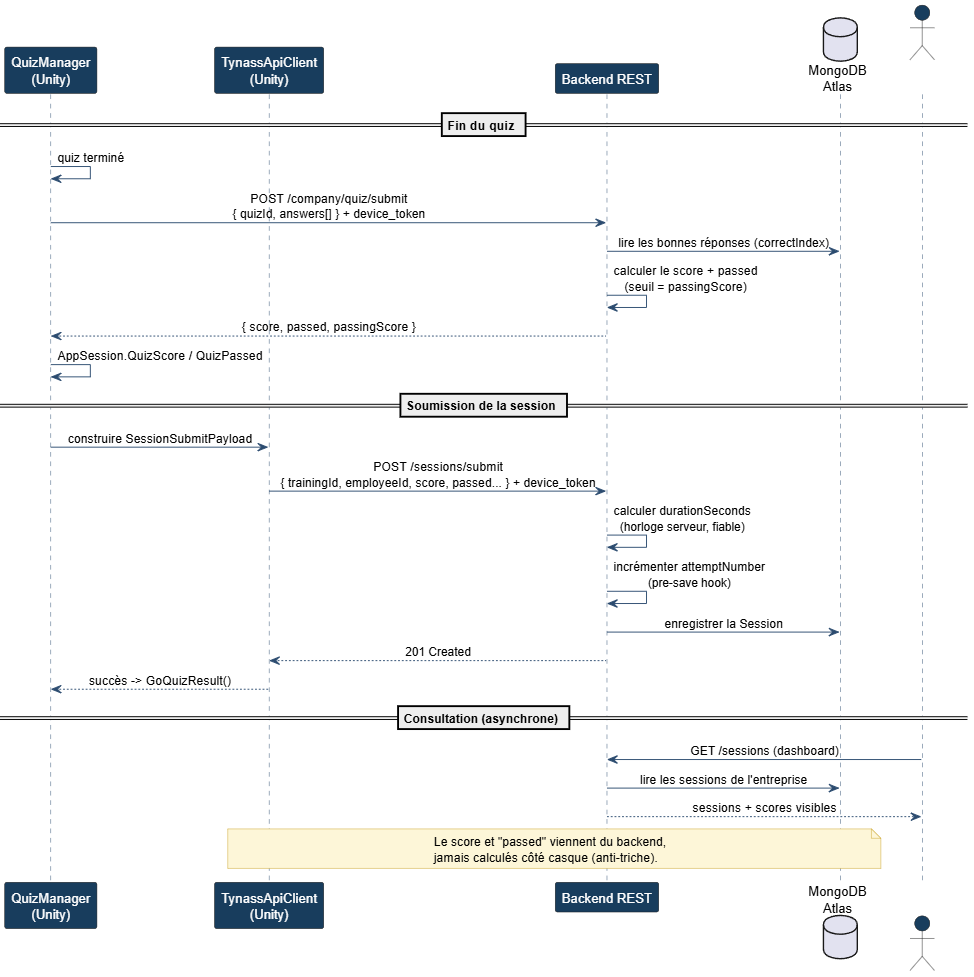
\includegraphics[width=0.9\textwidth]{../images/seqSubmit.png}
  \caption{Diagramme de séquence --- soumission d'une session}
  \label{fig:seq_submit}
\end{figure}

\section{Implémentation de l'itération~4}

Cette section détaille la mise en œuvre de la simulation~: les gestionnaires
d'orchestration et de quiz, puis le panneau d'affichage des résultats.

\subsection{OnboardingManager.cs et QuizManager.cs}

\texttt{OnboardingManager} orchestre l'exploration des huit zones (Phase~1). À la
fin de cette séquence, il délègue au \texttt{QuizManager} le déclenchement du quiz
(Phase~2) et la soumission finale des résultats~:

\begin{lstlisting}[language={[Sharp]C}, caption={QuizManager --- fin du quiz et SubmitSession}]
private async Task EndQuizAsync() {
    quizActive = false;
    quizPanel.SetActive(false);

    // Pourcentage, jamais le nombre brut de bonnes reponses
    AppSession.QuizScore = Mathf.RoundToInt(
        AppSession.QuizCorrect * 100f / AppSession.QuizTotal);
    bool passed = AppSession.QuizScore >= AppSession.PassingScore;

    string deviceToken = AppSession.DeviceToken;
    if (string.IsNullOrEmpty(deviceToken))
        deviceToken = PlayerPrefs.GetString("device_token", "");

    var result = await TynassApiClient.Instance.SubmitSession(
        trainingId:  AppSession.ActiveTraining?._id,
        employeeId:  AppSession.IsGuest ? null : AppSession.EmployeeId,
        startedAt:   AppSession.SimulationStartedAt,
        completedAt: DateTime.UtcNow,
        score:       AppSession.QuizScore,
        passed:      passed,
        deviceToken: deviceToken
    );

    if (result == null)
        Debug.LogError("SubmitSession a echoue");

    PanelManager.Instance.GoQuizResult();
}
\end{lstlisting}

\subsection{Panel QuizResult}

Le panel QuizResult affiche~:
\begin{itemize}
  \item Le score final en pourcentage.
  \item Le \textbf{statut}~: \og Réussi \fg{} (vert) ou \og Échoué \fg{} (rouge).
  \item Le détail des \textbf{critères d'évaluation} (procédure, identification,
    décision, temps).
  \item Un bouton \og Retour aux formations \fg{} et un bouton \og Se déconnecter \fg{}.
\end{itemize}

\placeholder{Capture Panel QuizResult --- score et critères (à insérer)}

\section{Difficultés et solutions}

\begin{table}[H]
  \centering
  \begin{tabularx}{\textwidth}{lXX}
    \toprule
    \textbf{Défi} & \textbf{Problème} & \textbf{Solution} \\
    \midrule
    Optimisation polygones & L'environnement complet dépassait
                             500\,000 polygones, causant des chutes
                             de FPS sur Meta Quest~3. &
                             Décimation des meshes dans Blender,
                             activation du LOD Group pour les
                             objets distants. \\
    \midrule
    Artefacts lightmap & Les baked lightmaps calculées dans Blender
                         n'étaient pas transférées correctement en
                         FBX vers Unity. &
                         Recalcul des lightmaps directement dans Unity
                         avec la Progressive Lightmapper. \\
    \midrule
    Timer quiz & La synchronisation entre QuizElapsedSecs et
                 les transitions de questions causait des décalages. &
                 Timer géré dans AppSession avec
                 \texttt{Time.deltaTime} indépendant des transitions. \\
    \bottomrule
  \end{tabularx}
  \caption{Difficultés rencontrées et solutions --- Itération~4}
  \label{tab:dificultes_s4}
\end{table}

\section{Évaluation de l'itération~4}

\begin{table}[H]
  \centering
  \begin{tabularx}{\textwidth}{Xl}
    \toprule
    \textbf{Élément validé} & \textbf{Statut} \\
    \midrule
    Exploration des 8 zones (7 départements + responsable) & Fonctionnel \\
    Narrations audio intégrées à la scène & Fonctionnel \\
    Quiz à choix multiples, score calculé côté backend & Fonctionnel \\
    Soumission automatique de session (\texttt{SubmitSession}) & Validé \\
    Session visible dans le dashboard d'administration & Validé \\
    Taille de l'APK & 2,4~Go \\
    \bottomrule
  \end{tabularx}
  \caption{Validation fonctionnelle --- Itération~4}
  \label{tab:eval_s4}
\end{table}

\placeholder{Capture environnement 3D Indigo dans Unity (à insérer)}

\placeholder{Capture quiz en VR --- question à choix multiples (à insérer)}

\placeholder{Capture session visible dans le dashboard admin (à insérer)}

\section{Conclusion}

Cette quatrième itération constitue le cœur du module de formation Indigo~:
modélisation complète de l'environnement 3D, narrations intégrées à la scène, système
de quiz fonctionnel et soumission automatique des résultats via \texttt{SubmitSession}.
Restent à finaliser la validation des tests sur casque et la mesure des métriques de
performance. Une fois ces vérifications effectuées, la simulation d'intégration d'Indigo
Company couvrira l'intégralité du parcours~: de l'exploration immersive des locaux
jusqu'à la remontée automatique des résultats dans le dashboard d'administration. Le
chapitre suivant présente la conclusion générale et les perspectives du projet.
